% -----------------------------------------------------------------------------
% Trabalhos Relacionados
% -----------------------------------------------------------------------------

\chapter{Granular Materials}
\label{chap:Trabalhos-Relacionados}

%Cada capítulo deve conter uma pequena introdução (tipicamente, um ou dois parágrafos), em seção não numerada, que deve deixar claro o objetivo e o que será discutido no capítulo, bem como a organização do capítulo.

%    Materiais granulares são conjunto de corpos sólidos, que individualmente podem ser compostos de um mesmo material ou de diferentes materiais, de geometria das mais variadas, podendo ter várias densidades, coeficiente de atrito, dureza, e várias outras propriedades físicas que os materiais possuem, mas todos são maiores que $100\mu m$, e portanto visíveis a olho nu \cite{Sands_Powders_and_Grains}. Interagem entre si quando estão em contato uns com os outros, perdendo energia, tanto na forma de dissipação inelástica, quanto no atrito entre os grãos.
%    Os corpos sólidos que constituem os materiais granulares são grandes o suficiente para não apresentarem influência cinemática em função da temperatura termodinâmica. Assim sendo, movimentos Brownianos são ausentes nesse tipo de sistema.

    Granular Materials are sets of solid bodies, which individually can be composed by same material or different materials. They can have variety geometry, different densities, friction coefficient, hardness, etc., but an individual grain must be larger than $100\mu m$ \cite{Sands_Powders_and_Grains} due to the athermous nature. The solid bodies that composes granular materials are large enough to do not present kinetic fluctuation induced by thermodynamic temperature. Therefore, Brownian motion do not appear in those systems. Granular materials interact each other when they are in contact, loosing energy in inelastic collision\footnote{Inelastic collision is a loss of kinetic energy due to the contact of the bodies, in which they have transformed part of the energy to heat and they may deform in the process \cite{Halliday}. We are modeling the inelastic collision between two grains in section \ref{subsubchap:Reologia}.}, as well as friction.

%    Segundo a \href{http://webofknowledge.com}{\textit{Web of Science}}, o número de produções publicadas com a palavra chave \textit{"Granular Materials"}, até $03/04/2018$, é de $8.618$ e segue a distribuição apresentada na figura \ref{fig:articles-year} ao longo dos anos. O estudo de materiais granulares também segue uma tendência crescente ao longo dos anos.
    
%\begin{figure}
%    \centering
%    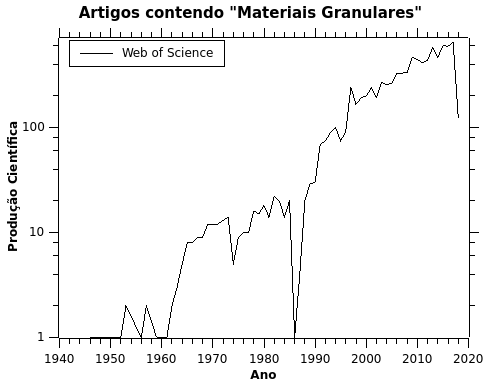
\includegraphics[width=0.8\textwidth]{04-figuras/articles-year.png}
%    \caption{Produção científica acerca de materiais granulares com as palavras chave \textit{"Granular Materials"} ao longo dos anos.}
%    \label{fig:articles-year}
%\end{figure}

\section{Theory}
\label{subsection:Teoria}

%    Como exemplos de materiais granulares temos areia, pedras, solos, fármacos, minérios, alimentos em grãos (arroz, milho, soja, etc.), e até mesmo o cinturão de asteroides e os anéis de Saturno. Só a areia compõe $10\%$ dos materiais da superfície do planeta Terra. Além disso, estima-se que o segundo material mais utilizado nas indústrias são materiais granulares, utilizando aproximadamente $10\%$ de toda a energia do planeta, sendo que o material mais utilizado é a própria água \cite{Sands_Powders_and_Grains}.

    Examples of granular materials includes sand, stones, soils, drugs, ores, grain foods (rice, corn, soybeans, etc.), even the asteroid belt and Saturn's rings. The sand alone makes up $10\%$ of the materials on surface of planet Earth. Besides that, it is estimated that the second most used material in industries are granular materials, using approximately $10\%$ of all the energy on the planet, with the most used material being water itself \cite{Sands_Powders_and_Grains}.

    \begin{figure}
        \begin{minipage}{.45\linewidth}
            \centering
            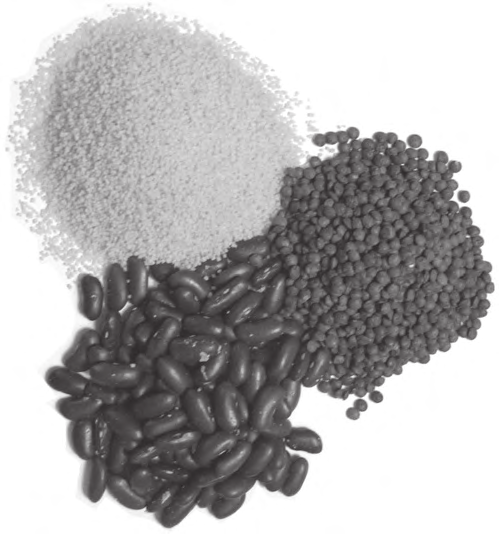
\includegraphics[width=0.9\textwidth]{04-figuras/Exemplo_Alimento.png}
            \subcaption{Grain foods.}
            \label{subfig:exemplo_alimento}
        \end{minipage}
        \begin{minipage}{.45\linewidth}
            \centering
            
\includegraphics[width=0.9\textwidth]{04-figuras/Exemplo_Medicamento.png}
            \subcaption{Drugs.}
            \label{subfig:exemplo_medicamento}
        \end{minipage}
        \begin{minipage}{.45\linewidth}
            \centering
            \includegraphics[width=0.9\textwidth]{04-figuras/Exemplo_Açucar.png}
            \subcaption{Sugar.}
            \label{subfig:exemplo_acucar}
        \end{minipage}
        \begin{minipage}{.45\linewidth}
            \centering
            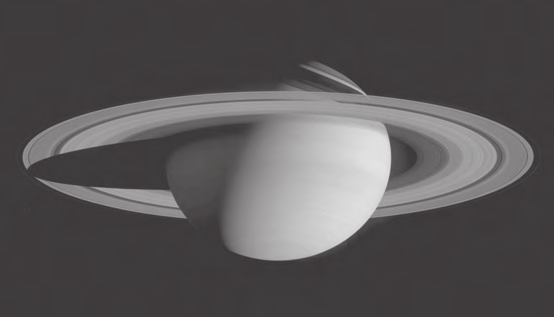
\includegraphics[width=0.9\textwidth]{04-figuras/Exemplo_Saturno.png}
            \subcaption{Saturn and its rings.}
            \label{subfig:exemplo_saturno}
        \end{minipage}
        \caption{Examples of granular material. Figures taken from \cite{Granular_Media_Between_Fluid_and_Solid}.}
    \end{figure}

%    Pela ausência de movimentos Brownianos, bem como pela dissipação de energia, sistemas granulares não sofrem relaxação espontânea de suas configurações estáveis na ausência de perturbações externas, principalmente na forma de vibrações, e portanto não apresentam ergodicidade\footnote{Um sistema ergódico tem característica de transitar entre seus microestados de energia espontaneamente, em intervalos de tempos, implicando que seus estados são todos equiprováveis quando analisados em um longuíssimo tempo \cite{Dissertacao, Srdjan-Tese, Granular_Solids_Liquids_and_Gases}.}.

    Due to the absence of Brownian movements, as well as the dissipation of energy in the contact, granular systems does not undergo spontaneous relaxation of its stable configurations in the absence of external disturbances, and therefore do no have ergodicity\footnote{An ergodic system has the characteristic of moving between their micro-states of energy spontaneously, in intervals of time, implying that their states are all equiprobable when analyzed in a very long time \cite{Srdjan-Tese, Unifying_Concepts_in_Granular_Media_and_Glasses}.}.

    To demonstrate this non-ergodicity, we can think about a dry sand pile that rests at a base. If this base does not oscillate, the structure of the pile does not change, the structure of internal forces will remain unchanged, even if it is heated or cooled. This means that sand grains cannot transit between all equipotential states spontaneously, and than this sand pile will rest with internal configurations (chain-forces, stress tensors, grain contact, etc.) unchanged. In the section \ref{subchap:Fenomenologia}, one can find more details.

%    Materiais granulares apresentam também particularidades quanto às suas fases. Apresentam-se individualmente em corpos sólidos, e quando o conglomerado está próximo do repouso, constituem a fase sólida do sistema. Porém, se o sistema é agitado, ou configurado além de um limiar crítico do ângulo de repouso, pode apresentar-se nas fases de granular líquido\footnote{Granulares líquidos podem possuir uma camada limite que flui sobre a camada sólida do sistema.} ou granular gasoso. Tal classificação ainda está em aberto na literatura, apesar de existirem proposições para o que seria a temperatura granular do sistema \cite{Granular_Solids_Liquids_and_Gases}.

    Granular materials also have particularities regarding their phases, analogously to the state of matter. They are presented individually in solid bodies, and when the conglomerate is close to rest, they constitute the equivalent solid phase of the state of matter. However, if the granular system is slightly agitated, or configured beyond a critical threshold of angle of rest, it can be interpreted in similarity of the liquid state of matter\footnote{Liquid granules can have a boundary layer that flows over the sold layer of the system.}. Granular gases are granular systems that are vigorously agitated, with low packing fraction\footnote{Packing fraction is the measure of the occupied space by the solid portion in relation of the total space.}, and they tend to occupy a large part of the recipe which contains them. An example of the granular state is shown in figure \ref{fig:exemplo_fases}, where the solid phase is static in the bottom, the liquid phase is flowing though layers in the middle, and the gaseous phase is flowing in a higher disordered portion at top. Such classification is still open in the literature, although there are proposals for what would be the granular temperature of the system, in analogous of thermal temperature \cite{Granular_Solids_Liquids_and_Gases}.

    \begin{figure}
        \centering
        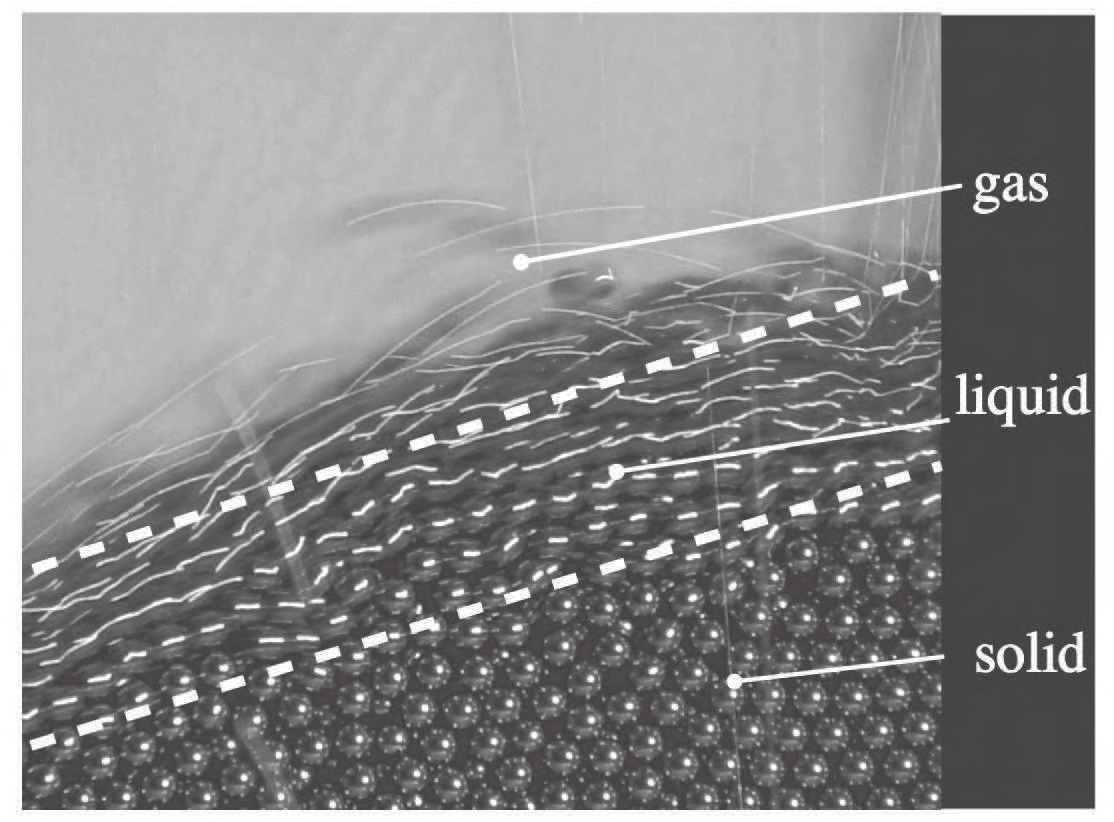
\includegraphics[width=0.9\textwidth]{04-figuras/Exemplo_Fases.png}
        \label{fig:exemplo_fases}
        \caption{Example of three granular phases according their kinetic energy. Figures taken from \cite{Granular_Media_Between_Fluid_and_Solid}.}
    \end{figure}

%    Uma diferenciação entre sistemas granulares pode ser resultado direto das forças de interações entre os grãos. São chamados de granulares secos os sistemas que possuem apenas interações repulsivas, enquanto os granulares molhados apresentam forças de van der Waals nas interações grão a grão. Nesta tese, consideraremos apenas as interações repulsivas de contato, apesar de que em alguns casos, existe fluido envolvendo o material. Consideramos que todo o material que está envolvido pelo mesmo fluido não sofre forças de atração entre os mesmos grãos, e portanto, não está inclusa força de van der Waals na interação entre os grãos.

    A differentiation between granular systems can be a direct result of the interaction forces between grains. Systems that have only repulsive interactions are called dry granulars, while wet granulars have van der Waals forces in grain-to-grain interactions. In this thesis, we will only consider repulsive contact interactions, although in some cases, there is fluid surrounding the material. We consider that all the material that is involved by the same fluid does not suffer forces of attraction between the same grains, and therefore, van der Waals force is not included in the interaction between the grains.

\section{Fenomenologia de Materiais Granulares}
\label{subchap:Fenomenologia}

%Pilha de areia
    Talvez a primeira ideia sobre materiais granulares remeta ao empilhamento de areira. Nesse caso, tem-se uma pilha estática de areia\footnote{A pilha estática está no estado sólido da fase granular \cite{Granular_Solids_Liquids_and_Gases}.}, amontoada sobre uma superfície. Note que em uma pilha como essa, os grãos sempre atingem uma determinada altura, e quando coloca-se mais material sobre a pilha, em algum momento, as camadas superiores da pilha escorrem até a base. Sempre que a pilha ultrapassar o ângulo crítico de repouso \cite{Granular_Physics}, ocorrerá uma avalanche, restaurando o sistema a um outro ângulo característico. Esta propriedade é a de auto-organização\footnote{Um sistema que não possui controlador central, regido por vários agentes que interagem entre si, com regras conhecidas na interação dos agentes e exibem propriedade não prevista pelas interações entre os agentes caracterizam um Sistema Complexo. Uma propriedade característica de Sistemas Complexos e de materiais granulares é a auto-organização. Alguns autores \cite{Mixing_and_Segregation_of_Granular_Materials, Measuring_the_flowing_properties_of_powders_and_grains, Revisiting_localized_deformation_in_sand_with_complex_systems, Granular_matter_and_networks, Patterns_and_collective_behavior_in_granular_media} classificam materiais granulares dentro da área de estudo de Sistemas Complexos.} da pilha de areia pelo ângulo crítico de repouso. Uma boa aproximação do ângulo de repouso é dada pela equação \ref{equ:atrito}:
\begin{equation}
    \label{equ:atrito}
    tan(\theta) = \mu _s ,
\end{equation}
onde $\theta$ é o ângulo crítico de repouso, e $\mu _s$ é o coeficiente de atrito do material.

%Biestabilidade da pilha
    Um pouco mais curioso ainda sobre as pilhas de grãos é que o histórico de preparação do sistema reflete-se no ângulo de repouso \cite{Dynamics_at_the_angle_of_repose}. Este histórico de preparação permite o sistema configurar-se diferentemente, e portanto, o ângulo de repouso assume valores diferentes utilizando o mesmo material. Existe então um ângulo de repouso mínimo $\theta _r$, e um ângulo máximo $\theta _m$, em que o empilhamento pode configurar-se: $\theta _r < \theta < \theta _m$ \cite{Granular_Physics}. Ter uma faixa de ângulos estáveis entre o ângulo mínimo de repouso e o ângulo máximo recebe o nome de biestabilidade do ângulo de repouso.

%Diferentes preparações, diferentes pressões
    Uma evidência de que o histórico de preparação altera a configuração do material é descrita nos artigos "\textit{Sensitivity of Stress Response Function to Packing Preparation}" e "\textit{Memories in sand: Experimental tests of construction history on stress distributions under sandpiles}" \cite{Sensitivity_of_Stress_Response_Function_to_Packing_Preparation, Memories_in_Sand}. A base circular apresentada na figura \ref{fig:pile_stress} foi feita com duas formas de deposição diferentes. No experimento, a pressão medida na base varia de acordo com a deposição, sendo que a deposição feita a partir do funil possui um pico de máximo de pressão em torno de $0,25$ e $0,5$ do raio da mesa, enquanto na deposição feita a partir da peneira apresenta pressão como espécie de platô entre o centro da mesa e $0,25$ do raio, com o máximo próximo do centro.

\begin{figure}
    \centering
    \begin{minipage}{.45\linewidth}
        \centering
        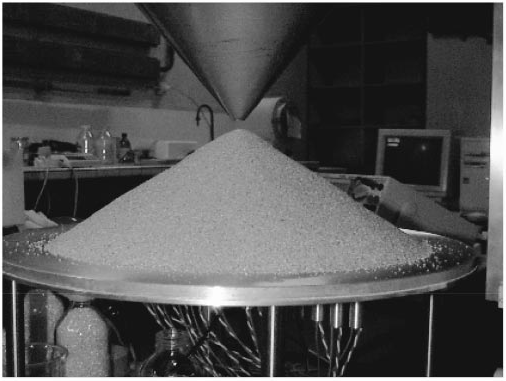
\includegraphics[width=0.9\textwidth]{04-figuras/Sand_Pile_GG_Experiment.png}
        \subcaption{Empilhamento a partir do funil.}
        \label{fig:pressure_pile:GG}
    \end{minipage}
    \begin{minipage}{.45\linewidth}
        \centering
        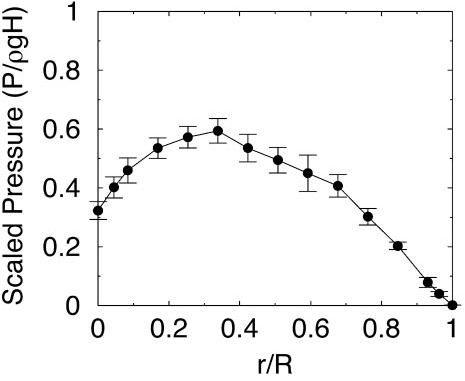
\includegraphics[width=0.9\textwidth]{04-figuras/Sand_Pile_GG_Pressure.png}
        \subcaption{Pressão na montagem a partir do funil.}
        \label{fig:pressure_response:GG}
    \end{minipage}
    \begin{minipage}{.45\linewidth}
        \centering
        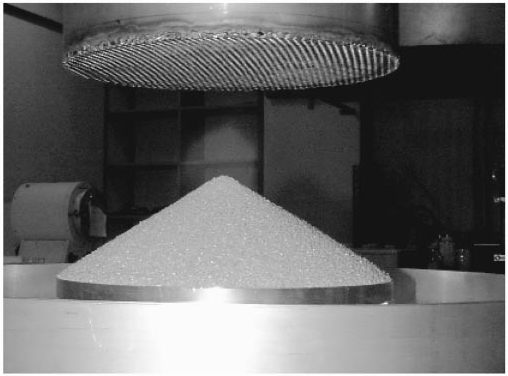
\includegraphics[width=0.9\textwidth]{04-figuras/Sand_Pile_RL_Experiment.png}
        \subcaption{Empilhamento a partir da peneira.}
        \label{fig:pressure_pile:RL}
    \end{minipage}
    \begin{minipage}{.45\linewidth}
        \centering
        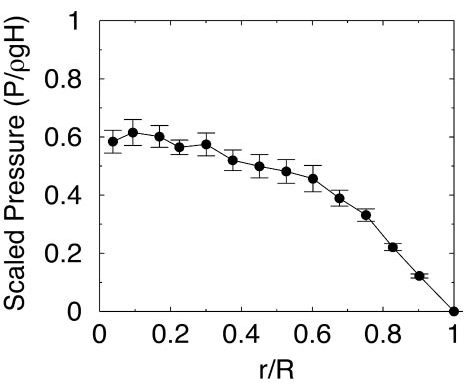
\includegraphics[width=0.9\textwidth]{04-figuras/Sand_Pile_RL_Pressure.png}
        \subcaption{Pressão na montagem a partir da peneira.}
        \label{fig:pressure_response:RL}
    \end{minipage}
    \caption{A preparação das pilhas de areia reflete nas pressões medidas na base da pilha. Nas figuras \ref{fig:pressure_pile:GG} e \ref{fig:pressure_response:GG} a deposição a partir do funil cria um perfil de pressões que tem o pico fora do centro da pilha, enquanto nas figuras \ref{fig:pressure_pile:RL} e \ref{fig:pressure_response:RL} a deposição a partir da peneira cria um perfil de pressões que tem um platô e depois decai. Figuras retiradas de \cite{Memories_in_Sand}.}
    \label{fig:pile_stress}
\end{figure}    

%Função resposta em diferentes configurações
    Um estudo feito por Atman \textit{et al.} \cite{Sensitivity_of_Stress_Response_Function_to_Packing_Preparation} mostra que diferentes geometrias de materiais granulares resultam em diferentes funções respostas\footnote{Função resposta é a diferença entre duas configurações, uma antes de aplicar-se a carga de teste e após a aplicação da carga, mostrando-se a distribuição de forças sobre o material, ou a compressão do sistema \cite{The_Physics_of_Granular_Media}.}. Como exemplo, a figura \ref{fig:stress_response} mostra duas funções respostas para sistemas com geometria circular e pentagonal.

\begin{figure}
    \centering
    \begin{minipage}{.45\linewidth}
        \centering
        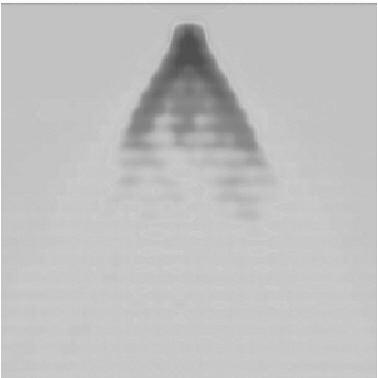
\includegraphics[width=0.9\textwidth]{04-figuras/Funcao_Resposta1.png}
        \subcaption{Grãos circulares.}
        \label{fig:stress_response:circle}
    \end{minipage}
    \begin{minipage}{.45\linewidth}
        \centering
        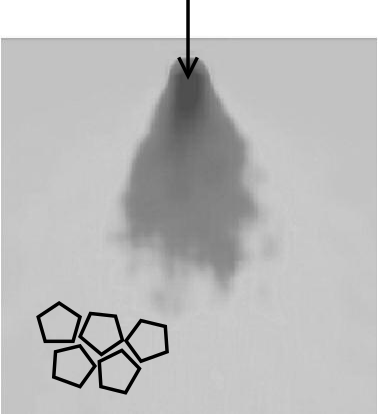
\includegraphics[width=0.9\textwidth]{04-figuras/Funcao_Resposta2.png}
        \subcaption{Grãos pentagonais.}
        \label{fig:stress_response:pentagon}
    \end{minipage}
    \caption{A aplicação de uma força em diferentes sistemas granulares resulta em diferentes funções respostas. A diferença entre estes sistemas é que a figura \ref{fig:stress_response:circle} possui grãos de geometria circular e possui maior ordem, enquanto a figura \ref{fig:stress_response:pentagon} possui geometria pentagonal e maior desordem. Figuras retiradas de \cite{Sensitivity_of_Stress_Response_Function_to_Packing_Preparation}.}
    \label{fig:stress_response}
\end{figure}

%Cadeias de forças em diferentes pilhas
    Já que citamos as diferentes funções respostas nos empilhamentos de grãos, não podemos deixar de citar as cadeias de forças\footnote{Cadeias de forças consistem na rede de contatos entre os grãos que possuem força acima da força média do sistema. Em geral, mede-se as cadeias de forças são medidas a partir da função resposta \cite{The_Physics_of_Granular_Media}.}. A importância experimental da visualização das cadeias de forças se dá no entendimento da distribuição das forças internas que sustentam o material. Como exemplo, a figura \ref{fig:force_chain} indicia a cadeia de forças associada à função resposta de uma força puntual aplicada sobre o topo do material granular.

\begin{figure}
    \centering
    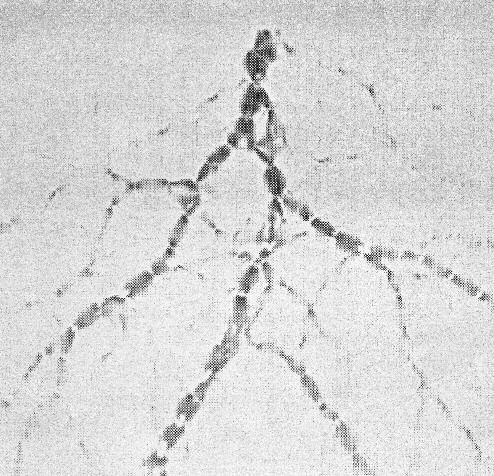
\includegraphics[width=0.5\textwidth]{04-figuras/Cadeia_Forca.png}
    \caption{A aplicação de uma força puntual no topo do material resulta na cadeia de forças, que pode ser vista através da função resposta do sistema. Neste caso, o sistema é preparado com grãos fotoelásticos em uma distribuição bidimensional. Quanto mais escuras, maiores são as tensões no material. Figura retirada de \cite{Sensitivity_of_Stress_Response_Function_to_Packing_Preparation}.}
    \label{fig:force_chain}
\end{figure}

%Formação de arcos
    As cadeias de forças são importantes para entender o fenômeno que está presente nos arcos de sustentação que utilizamos. Arcos são estruturas coletivas que possuem sustentação mútua, e, consequentemente, uma cadeia de forças ligando toda a estrutura, sendo capaz de sustentar o peso próprio e de todos os grãos acima, impedindo que os mesmos escoem. Na formação de arcos podem ocorrer efeitos de segregação, como verificado por Magalhães, C. e Magalhães, F. \cite{Caio-Tese, Felipe-Tese}.

%Pressão e tensão
    As medidas em materiais granulares geralmente tentam caracterizar o material em duas escalas diferentes que se relacionam: microescala, que diz respeito das medidas na escala dos grãos, como atrito; e macroescala, que diz respeito das medidas na escala do sistema, como pressão e tensão de cisalhamento.

%Dilatação
    Uma curiosidade sobre os materiais granulares é que quando estão submetidos a uma pressão e seu coeficiente de compactação\footnote{\label{foot:packingfraction}O coeficiente de compactação é dado pela razão da soma dos volumes individuais dos grãos pelo volume de ocupação no espaço.} está próximo do engarrafamento \cite{Non-Gaussian_behavior_in_jamming_unjamming_transition_in_dense_granular_materials}, uma dilatação tende a ocorrer, expandindo-se pelas bordas das fronteiras que confinam o material ou pelas outras direções de liberdade que o confinamento apresenta. Muitas vezes, ao aplicar-se uma pressão no material confinado, o coeficiente de compactação final pode ser menor que o inicial, indicando uma expansão volumétrica do sistema \cite{Felipe-Tese}.

%Escoamento de granular
    Aproveitando o exemplo do empilhamento, observa-se que na formação da pilha, após os grãos atingem o ângulo critico, ocasiona-se uma avalanche do material. Na avalanche, a camada superior entra em movimento, enquanto as camadas abaixo continuam estáticas. Na movimentação da camada superior, o material granular se apresenta no estado líquido, enquanto a camada estática abaixo encontra-se no estado sólido \cite{Granular_Solids_Liquids_and_Gases}. A figura \ref{fig:inclinacao} exemplifica a transição de fase sólido líquido entre as camadas.

\begin{figure}
    \centering
    \begin{minipage}{.45\linewidth}
        \centering
        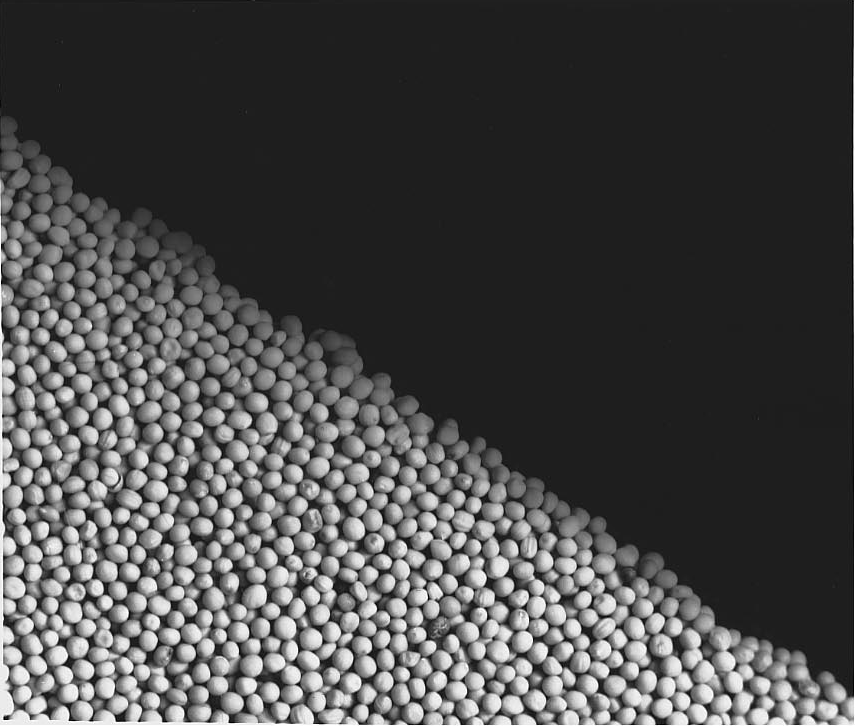
\includegraphics[width=0.9\textwidth]{04-figuras/Pilha1.png}
        \subcaption{Pilha estática.}
        \label{fig:inclinacao:solido}
    \end{minipage}
    \begin{minipage}{.45\linewidth}
        \centering
        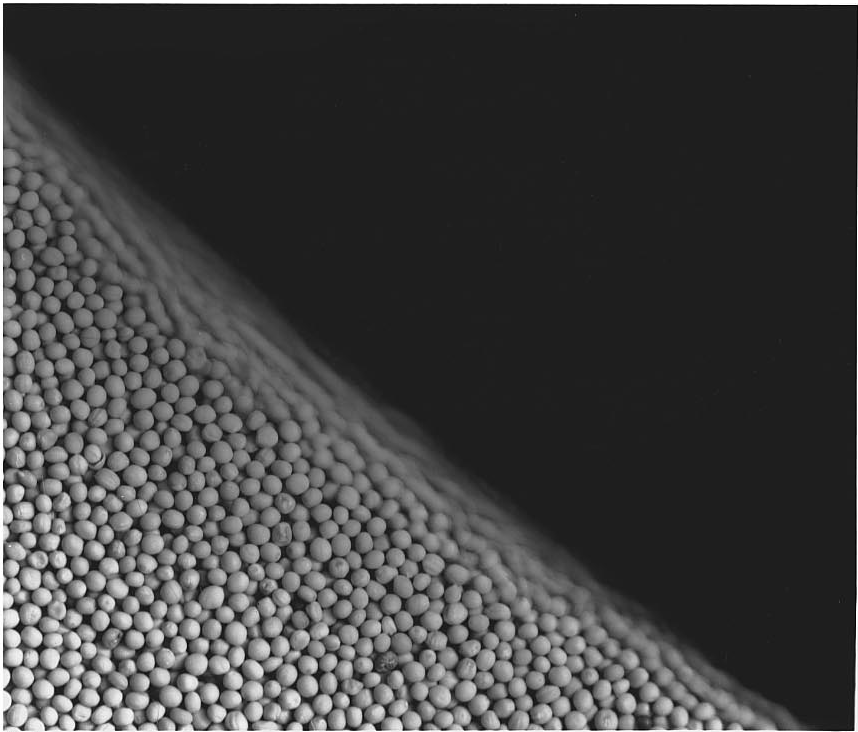
\includegraphics[width=0.9\textwidth]{04-figuras/Pilha2.png}
        \subcaption{Pilha escorrendo.}
        \label{fig:inclinacao:liquido}
    \end{minipage}
    \caption{Com o aumento do ângulo da pilha, nota-se que a camada superior desliza sobre a camada inferior (da figura \ref{fig:inclinacao:solido} para a figura \ref{fig:inclinacao:liquido}). Figuras retiradas de \cite{Granular_Solids_Liquids_and_Gases}.}
    \label{fig:inclinacao}
\end{figure}

    Escoamentos podem ocorrer então por tensões aplicadas no material, seja em uma inclinação da base, seja pela vibração do material. Como a mudança de configurações do material está relacionada a taxa de cisalhamento do material, mas a tensão de cisalhamento não é necessariamente proporcional a taxa de cisalhamento, este escoamento pode ser classificado como fluido não newtoniano.

%Segregação
%    Um fenômeno muito estudado é a segregação dos materiais granulares. O efeito de segregação ocorre em diferentes geometrias de material, densidades e coeficientes de atrito.

%Vibração
%    Vibrações no material granular fornecem energia ao sistema

    No próximo capítulo descreveremos as equações e os procedimentos para realizar as simulações dos materiais granulares, desde o modelo de contatos até a inserção do fluido no sistema.
